\newpage
\genHeader

\section{Get a simple demo running}


\begin{itemize}
\hypertarget{simpleDemo common}{} 
\item[$\blacktriangleright$]
Open Eclipse to a clean, fresh workspace.
Go to \menuPath{Window/Open Perspective/Other\ldots} \footnote{A path given as \menuPath{foo \menuSep bar} indicates how to navigate in a series of menus and toolbars.
New definitions or concepts will be \newconcept{italicized}, and any data you're required to enter, open, or select will be given as \filename{command}.} and choose \texttt{eMoflon} (\Cref{eclipse:openPerspective}).

\begin{figure}[htbp]
	\centering
  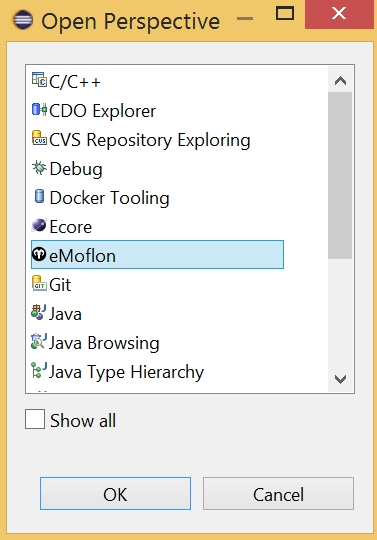
\includegraphics[width=0.5\textwidth]{eclipse_openPerspective}
	\caption{Choose the eMoflon perspective}
	\label{eclipse:openPerspective}
\end{figure} 

\item[$\blacktriangleright$] At either the far right or centre of the toolbar, a new action set should have appeared.
Navigate to \menuPath{Install Workspace \menuSep eMoflon Examples \menuSep Demo (Double-Linked List)} \LK{Please update the screenshot.}
(\Cref{eclipse:newMetamodel}).
%
\vspace{0.5cm}
\begin{figure}[htbp]
	\centering
  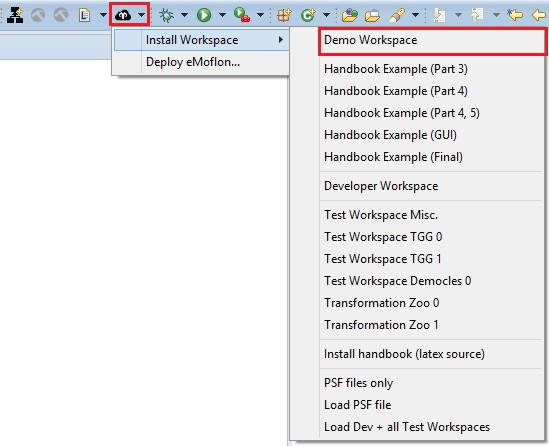
\includegraphics[width= 0.7\textwidth]{eclipse_MoflonButton}
	\caption{Invoking \enquote{Install Workspace $\to$ eMoflon Examples $\to$ Demo (Double-Linked List)}}
	\label{eclipse:newMetamodel}
\end{figure}

\newpage

\item[$\blacktriangleright$] In this menu you can check out different workspaces for Eclipse. Here you can also check out worspaces for the handbook tutorials. How you can create your own projects is described in Part I. As the first tutorial select ``Demo Workspace''. 

\item[$\blacktriangleright$]  Another button in the new action set is \menuPath{View and configure logging} represented by an \texttt{L} (\Cref{eclipse:logger}).
Clicking this icon will open a \texttt{log4jConfig.properties} file where you can silence certain loggers, set the level of loggers, or configure other
settings.\footnote{If you're not sure how to do this, check out a short Log4j tutorial a \url{http://logging.apache.org/log4j/1.2/manual.html}} All of eMoflon's
messages appear in our console window, just below your main editor. This is automatically opened when you selected the \texttt{eMoflon} perspective and
contains important information for us if something goes wrong!

\begin{figure}[htbp]
	\centering
  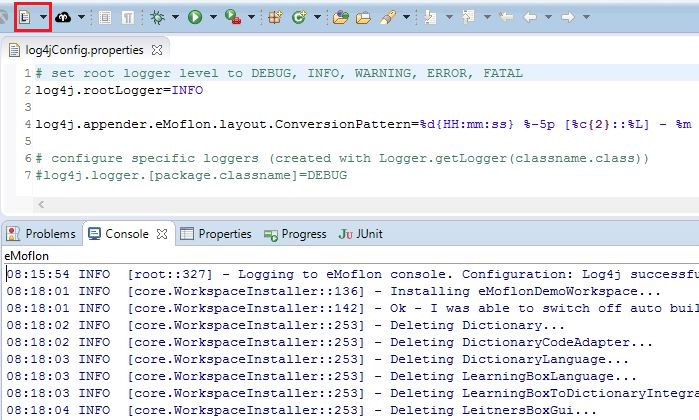
\includegraphics[width=\textwidth]{eclipse_logger}
	\caption{The eMoflon console with log messages}
	\label{eclipse:logger}
\end{figure} 
\end{itemize}

\clearpage
\visHeader

\subsection{A first look at Enterprise Architect}

\begin{itemize}
\FloatBarrier
\hypertarget{simpleDemo vis}{}
\item[$\blacktriangleright$] Can you locate the new \texttt{Demo.eap} file in your package explorer? This is the EA project file you'll be
modelling in. Don't worry any other folders at the moment - all problems will be resolved by the end of this section.

In the meantime, do not rename, move, or delete anything.

\item[$\blacktriangleright$] Double-click \texttt{Demo.eap} to start EA, and choose \texttt{Ultimate} when starting EA for the first time.

\item[$\blacktriangleright$] In EA, navigate to ``Extensions/MOFLON::Ecore Addin/Export\- all\- to\- Workspace'' (Fig.~\ref{fig:ea}). 

\begin{figure}[htbp]
	\centering
  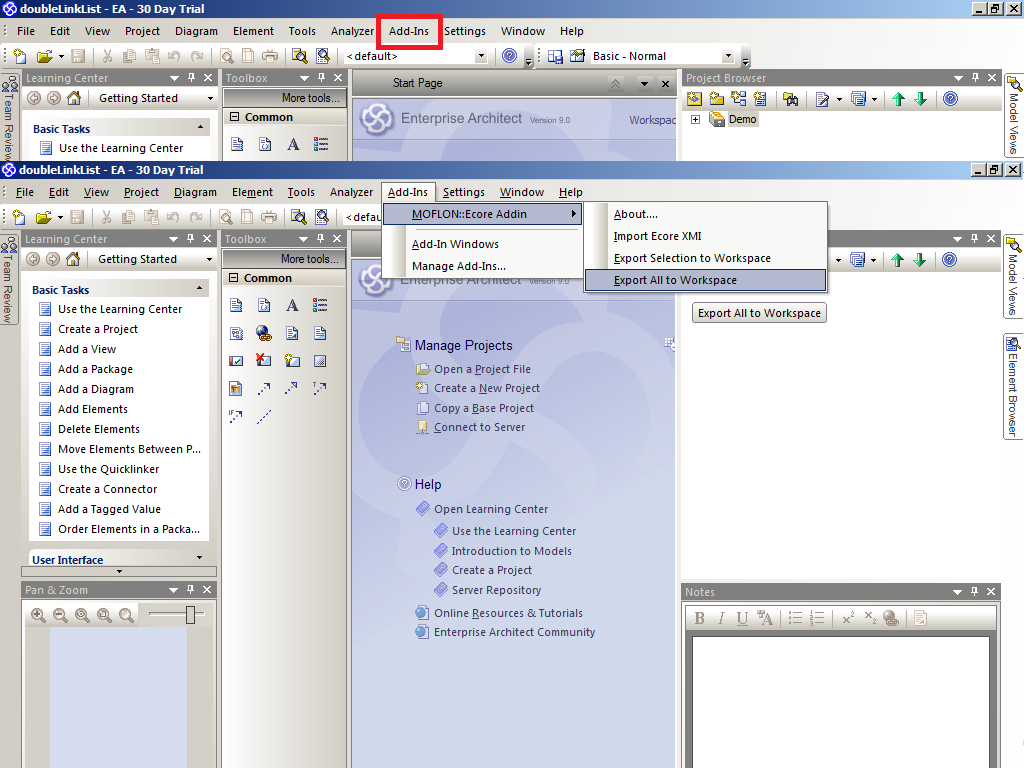
\includegraphics[width=0.9\textwidth]{ea_firststart}
	\caption{Export from EA} 
	\label{fig:ea} 
\end{figure}

\item[$\blacktriangleright$] Please note that this submenu is limited, and does not provide access to all eMoflon functionality. You can activate eMoflon's full
control panel window by going to ``Extensions/Add-In Windows'' (Fig.~\ref{fig:controlPanel}). To export from here, click \texttt{All} in the ``Export'' section.

\begin{figure}[htbp]
	\centering
  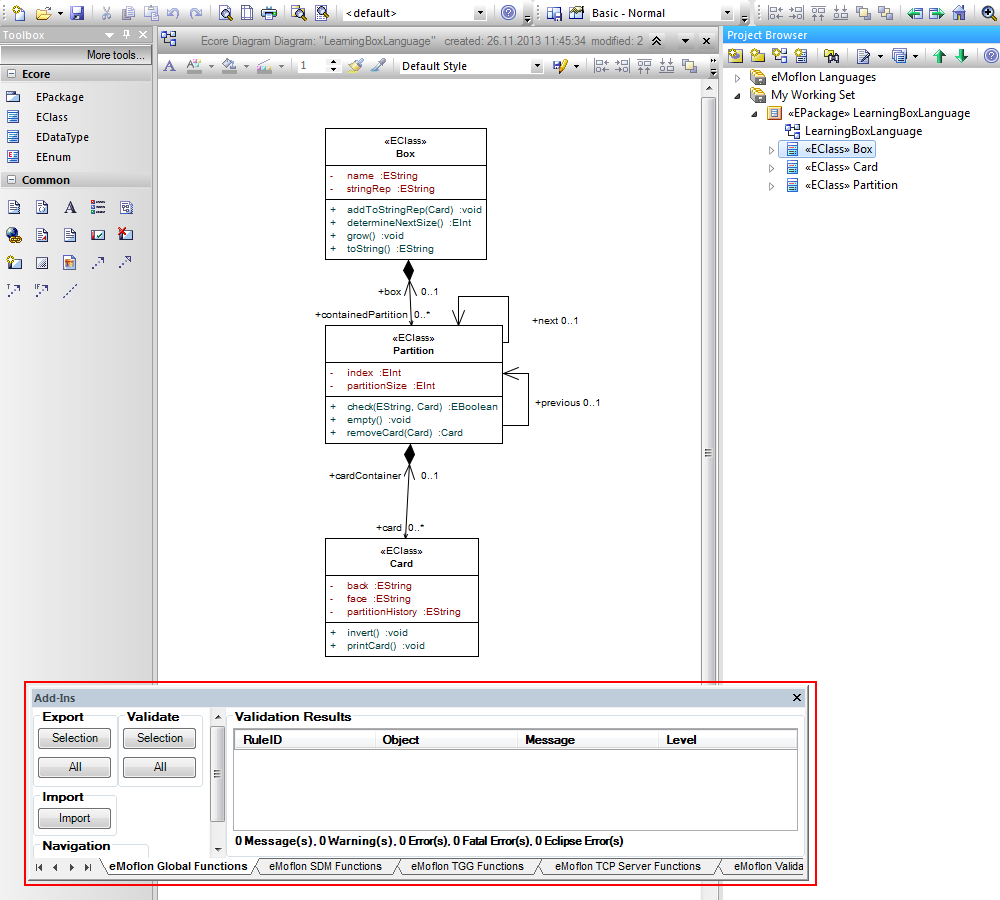
\includegraphics[width=0.9\textwidth]{ea_controlPanel}
	\caption{eMoflon's control panel} 
	\label{fig:controlPanel} 
\end{figure}

\item[$\blacktriangleright$] Now try exploring the EA project browser! Try to navigate to the packages, classes, and diagrams. Don't worry if you don't
understand that much - we'll get to explaining everything in a moment. Just make sure not to change anything!

%\nxtPage{\thepage}
\newpage

\item[$\blacktriangleright$] Switch back to Eclipse, choose your metamodel project, and press F5 to refresh. A new folder should appear, and your errors should
disappear after a few seconds. Since you've chosen to use our visual syntax, there isn't much to look at here. The export from EA places all required files in a
hidden folder(.temp) in the project, and refreshing triggers a build process that invokes our code generator automatically. 

\item[$\blacktriangleright$] You should be able to monitor the progress with the green bar in the lower right corner (Fig.~\ref{fig_eclipseBuild}). Pressing the
symbol opens a monitor view that gives more details of the build process. You don't need to worry about any of these details, just remember to refresh your
Eclipse workspace after an export.

\fancyfoot[OR]{$\triangleright$ \hyperlink{validate common}{Next}}

\begin{figure}[htbp]
	\centering
  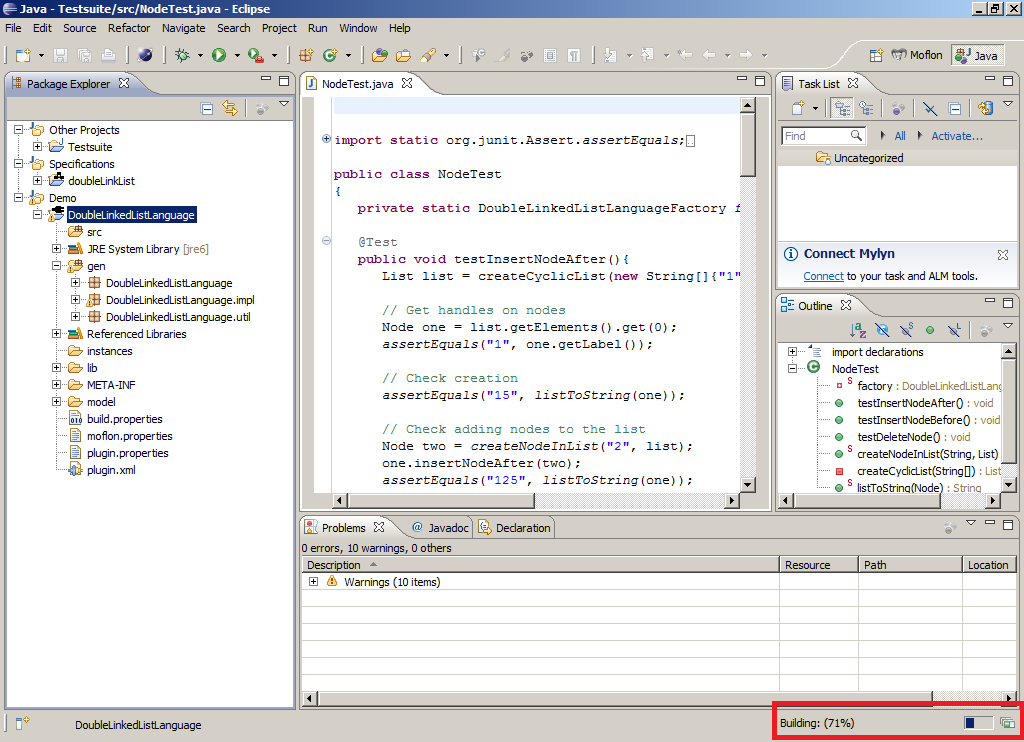
\includegraphics[width=0.9\textwidth]{eclipse_building}
	\caption{Eclipse workspace when using visual syntax} 
	\label{fig_eclipseBuild} 
\end{figure}

\item[$\blacktriangleright$] If you're ever worried about forgetting to refresh your workspace, or if you just don't want to bother with having to do this,
Eclipse does offer an option to do it for you automatically. To activate this, Go to ``Window/Preferences/General/Workspace" and select \texttt{refresh on
access}.

\end{itemize}

